\section*{Problema}

El área de un casquete esférico de la siguiente forma
	\begin{figure}[H]
		\centering
		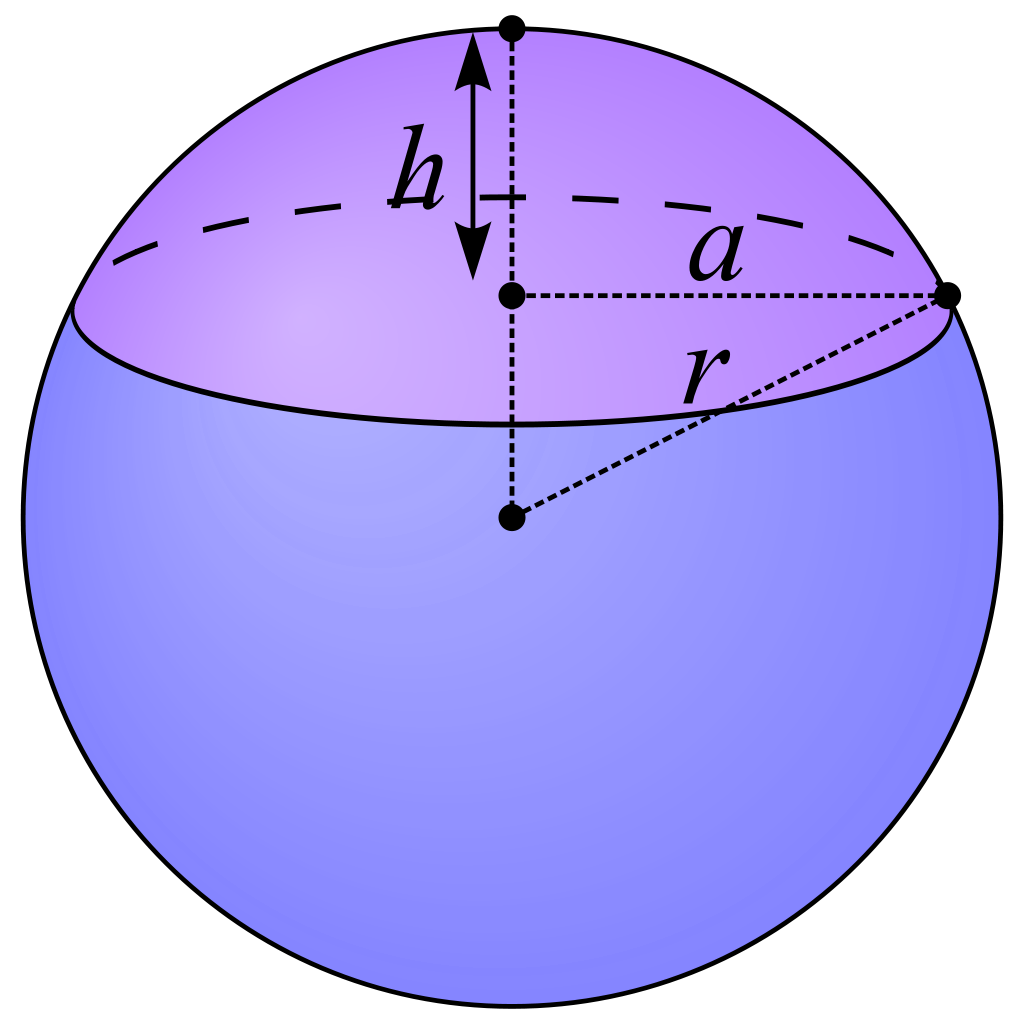
\includegraphics[scale=0.1]{./img/casquete.png}
		\caption{Casquete esférico.}
		\label{casq}
	\end{figure}
es: $ A = \pi (a^2 + h^2) \quad \Rightarrow \quad A = 2\pi r^2 \qty(1-\cos{\theta}) $. Con esto y teniendo el campo eléctrico de una carga puntual
	$$ \Phi _E = \qty[2\pi r^2 (1-\cos{\theta})]\qty[\frac{Q}{4\pi \varepsilon _o r^2}], $$
	$$ \Phi _E = \frac{Q}{2\varepsilon _o} (1 - \cos{\theta}). $$
Para $\theta = 90^o$:
	$$ \Phi _E (\theta = 90^o) = \frac{Q}{2\varepsilon _o} $$
flujo en una semiesfera. \\
Para $\theta = 180^o$:
	$$ \Phi _E (\theta = 180^o) = \frac{Q}{\varepsilon _o} $$
flujo en una esfera completa, el caso "base" de la ley de Gauss.










%%%%